\documentclass{article}
\usepackage{amsmath}
\usepackage{amsthm}
\usepackage{amsfonts}
\usepackage{amssymb}
\usepackage{bbold}
\usepackage{dsfont}
\usepackage{graphicx}
\usepackage{cleveref}
\usepackage{bm}
\usepackage{booktabs}
\usepackage{siunitx}
\usepackage{xcolor}
\usepackage{pdfpages}
\usepackage[utf8]{inputenc}
\usepackage[english]{babel}
\newtheorem{definition}{Definition}
\newtheorem{example}{Example}
\newcommand{\exP}[1]{\mathrm{e}^{#1}}
\newcommand{\dif}{\mathrm{d}}
\renewcommand{\vec}[1]{\mathbf{#1}}
\newcommand{\pdagger}{{\phantom{\dagger}}}
\newcommand{\state}[1]{\vert #1\rangle}
\newcommand{\cstate}[1]{\langle #1\vert}
\newcommand{\tr}[1]{\mathrm{tr}\left\{#1\right\}}
\newcommand{\trs}[2]{\, \mathrm{tr}_{#1}\{#2\}}
\newcommand{\expc}[3]{\langle #1\vert #2 \vert #3\rangle}
\usepackage[doi=false,url=false,isbn=false,backend=bibtex,style=nature,natbib=true,sorting=none]{biblatex}
\bibliography{bib.bib}
\usepackage{geometry}
\geometry{
	a4paper,
	total={170mm,257mm},
	left=15mm,
	right=15mm,
	top=15mm,
}
\begin{document}
\title{Singlet fission in o-TIPSm with spin-PLDM}
%\author{Rudolf Smorka}
\maketitle
\section{Model}\label{sec:Model}
The Hamiltonian used in \cite{reddy2018intramolecular} reads in the diabatic basis
\begin{equation}
	H = \sum_{I} H_I \vert I\rangle\langle I\vert + \sum_{I>J} (V_{IJ}\vert I\rangle \langle J\vert +\mathrm{h.c.}),
\end{equation}
where $I,J$ label different diabatic states. Here, $H_I$ is 
\begin{equation}
	H_I = E_I^0 + \sum_l \frac{\omega_l}{2}\left(Q_l^2 + P_l^2\right) + \sum_l \left(\kappa_{I,I}^l Q_l + \frac{1}{2}\gamma_{I,I}^l Q_l^2\right),\label{eq:HamI}
\end{equation}
and $V_{IJ}$ is
\begin{equation}
	V_{IJ} = V_{IJ}^0 + \sum_l \left(\kappa_{I,J}^l Q_l + \frac{1}{2}\gamma_{I,J}^l Q_l^2\right).\label{eq:HamIJ}
\end{equation}
Remarks:
\begin{itemize}
	\item The parameters in the file ortho-couplings-28-modes.inp are the same as in the input files used in the MCTDH calculations (which were used to produce the results shown in Fig. 3 in \cite{reddy2018intramolecular}). These are the correct parameters and should be used in the simulations.
	
	As discussed in the SI of \cite{reddy2018intramolecular}, a coordinate transformation has been performed, which affects energies and couplings. The values given in Table 2 in \cite{reddy2018intramolecular} and Tables S2-S11 (in SI) correspond to the model before the coordinate transformation, and should not be used directly. Also, there are some typos/errors in the table S12, so these values should not be used either.
	\item In the definition of the Hamiltonian, the state-dependent bilinear coupling term contains a factor $\frac{1}{2}$. One possible way to include it in the semiclassical calculations is in the definition of the Model class (system.py). 
	\item The correspondence between the physical state and its number in the MCTDH/spin mapping input file and the state number in the publication is the following:   
	\begin{table}[!h]
		\centering
%		\caption{Correspondence between state numbers in the input file for the MCTDH, spin-PLDM and spin-LSC calculations (first column), physical state, and state number in the tables in \cite{reddy2018intramolecular}.}
	\begin{tabular}{cc}
		\toprule
		(in MCTDH/spin mapping input) State & Number in \cite{reddy2018intramolecular}  \\ \midrule
		(1) $\vert ^1(S_0 S_0)\rangle$  & 1  \\
		(2) $\vert ^1(T_1 T_1)\rangle$ &  4  \\
		(3) $\vert ^1(S_1 S_0)\rangle$ & 3 \\
		(4) $\vert ^1(S_0 S_1)\rangle$ & 2 \\
		(5) $\vert ^1(AC)\rangle$ &  6 \\
		(6) $\vert ^1(CA)\rangle$ & 5 \\
		(7) $\vert ^1(DE_1)\rangle$ &  7  \\
		(8) $\vert ^1(DE_2)\rangle$ & 8  \\ \bottomrule
	\end{tabular}
	\end{table}
\end{itemize}
\clearpage
\section{Initial State}
The initial state in the MCTDH calculations is a product state 
\begin{equation}
	\vert \Psi_0\rangle = \vert I\rangle \vert 0_0\rangle,
\end{equation}
where $\vert I\rangle$ denotes the initially excited electronic state ($\vert ^1(S_1S_0)\rangle$ in the calculations, i.e. state number 3), and $\vert 0_0 \rangle$ denotes the vibrational ground state in the electronic ground state. This state is a product state over all vibrational modes $\vert 0_0\rangle =\vert 0_0^1\rangle \dots \vert 0_0^l\rangle\dots \vert 0_0^F\rangle$, and is obtained by diagonalizing the electronic ground state Hamiltonian
\begin{equation}
	H_{1}^l =  \frac{\omega_l}{2} P_l^2 + \frac{\omega_l+\gamma_{1,1}^l}{2}Q_l^2 \label{eq:InitialHam}
\end{equation}  
for each mode.
Note, that this is the same Hamiltonian as \cref{eq:HamI,eq:HamIJ} for the electronic ground state where we used the fact that linear couplings for this state vanish $\kappa_{1,1}^l=0$ for all modes.  

In the current implementation in the NRPMD code, the initial state is sampled from the Wigner distribution for the vibrational ground state in the vibrational Hamiltonian
\begin{equation}
	H_\mathrm{vib}^{l} = \frac{\omega_l}{2}\left(Q_l^2 + P_l^2\right)\label{eq:HO_Ham}
\end{equation}
for each mode. We still have to check this but we do not expect big changes.
\section{Full model}
In the spin-PLDM calculations, focused sampling of electronic mapping variables is used and the nuclei are sampled from the Wigner distribution at zero temperature with respect to \cref{eq:HO_Ham}. We checked out two integrators (velocity-Verlet and scipy.odeint), with both giving essentially the same results. Also, we checked that energy is conserved for a single trajectory for both integrators.  
Then, the first thing to check was the influence of the factor $\frac{1}{2}$ in the definition of the model in \cref{eq:HamI,eq:HamIJ} on the spin-PLDM calculations. The influence on the dynamics is negligible using this method, and therefore the results are not shown here. 

\Cref{fig:SpinPLDM_full_spinLSC} shows a comparison between spin-PLDM (velocity-Verlet, $10^6$ trajectories) and spin-LSC (with [green] and without [red] factor $\frac{1}{2}$, $10^5$ trajectories) with the MCTDH results (turquoise lines). 
There is good agreement only up to $\sim \SI{50}{\femto\second}$. 
The spin-PLDM results deviate strongly from the exact results for longer times, and populations get unphysical for $t>\SI{100}{\femto\second}$. 
Notable is also the influence of the factor $\frac{1}{2}$ in the model definition on the spin-LSC results. Including the factor leads to a larger deviation from the MCTDH results.      
\begin{figure}[!h]
	\centering
	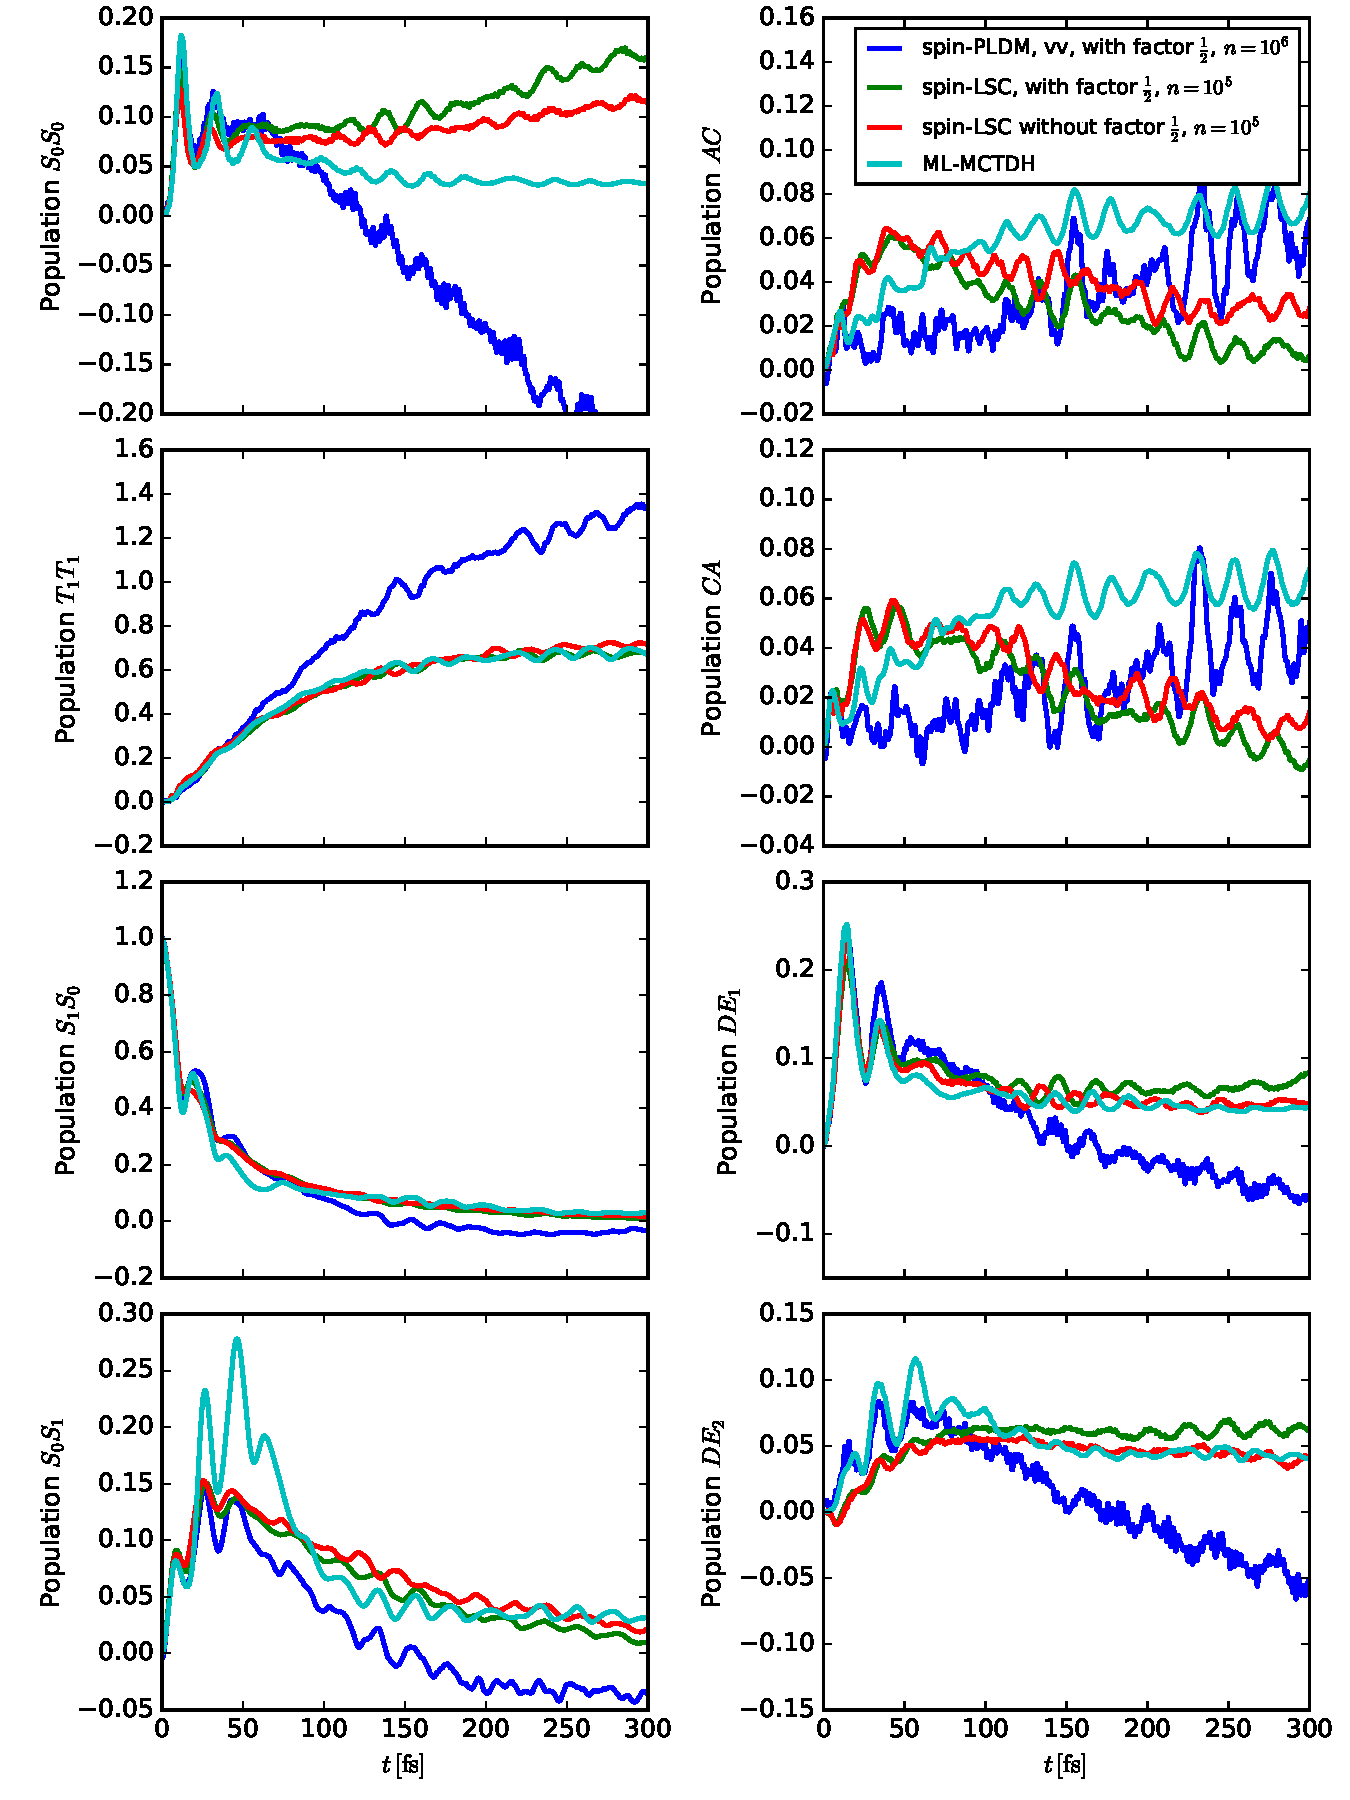
\includegraphics[width=0.9\textwidth]{figs/SF_comparison_multi_allStates_fixed_spinPLDM_spinLSC.pdf}
	\caption{Comparison of population dynamics: spin-PLDM vs spin-LSC (with and without factor $\frac{1}{2}$) vs MCTDH.}\label{fig:SpinPLDM_full_spinLSC}
\end{figure}
\clearpage
\section{Reduced model}
To further investigate the cause of negative populations in the spin-PLDM calculations, we investigate two reduced models: One in which the bilinear coupling is set to zero $\gamma_{I,J}^l = 0$ (\cref{fig:SpinPLDM_red_bilinear}) and another for the purely electronic system ($\gamma_{I,J}^l = 0$ and $\kappa_{I,J}^l = 0$, \cref{fig:SpinPLDM_red_nocoupl}). 

\begin{figure}[!h]
	\centering
	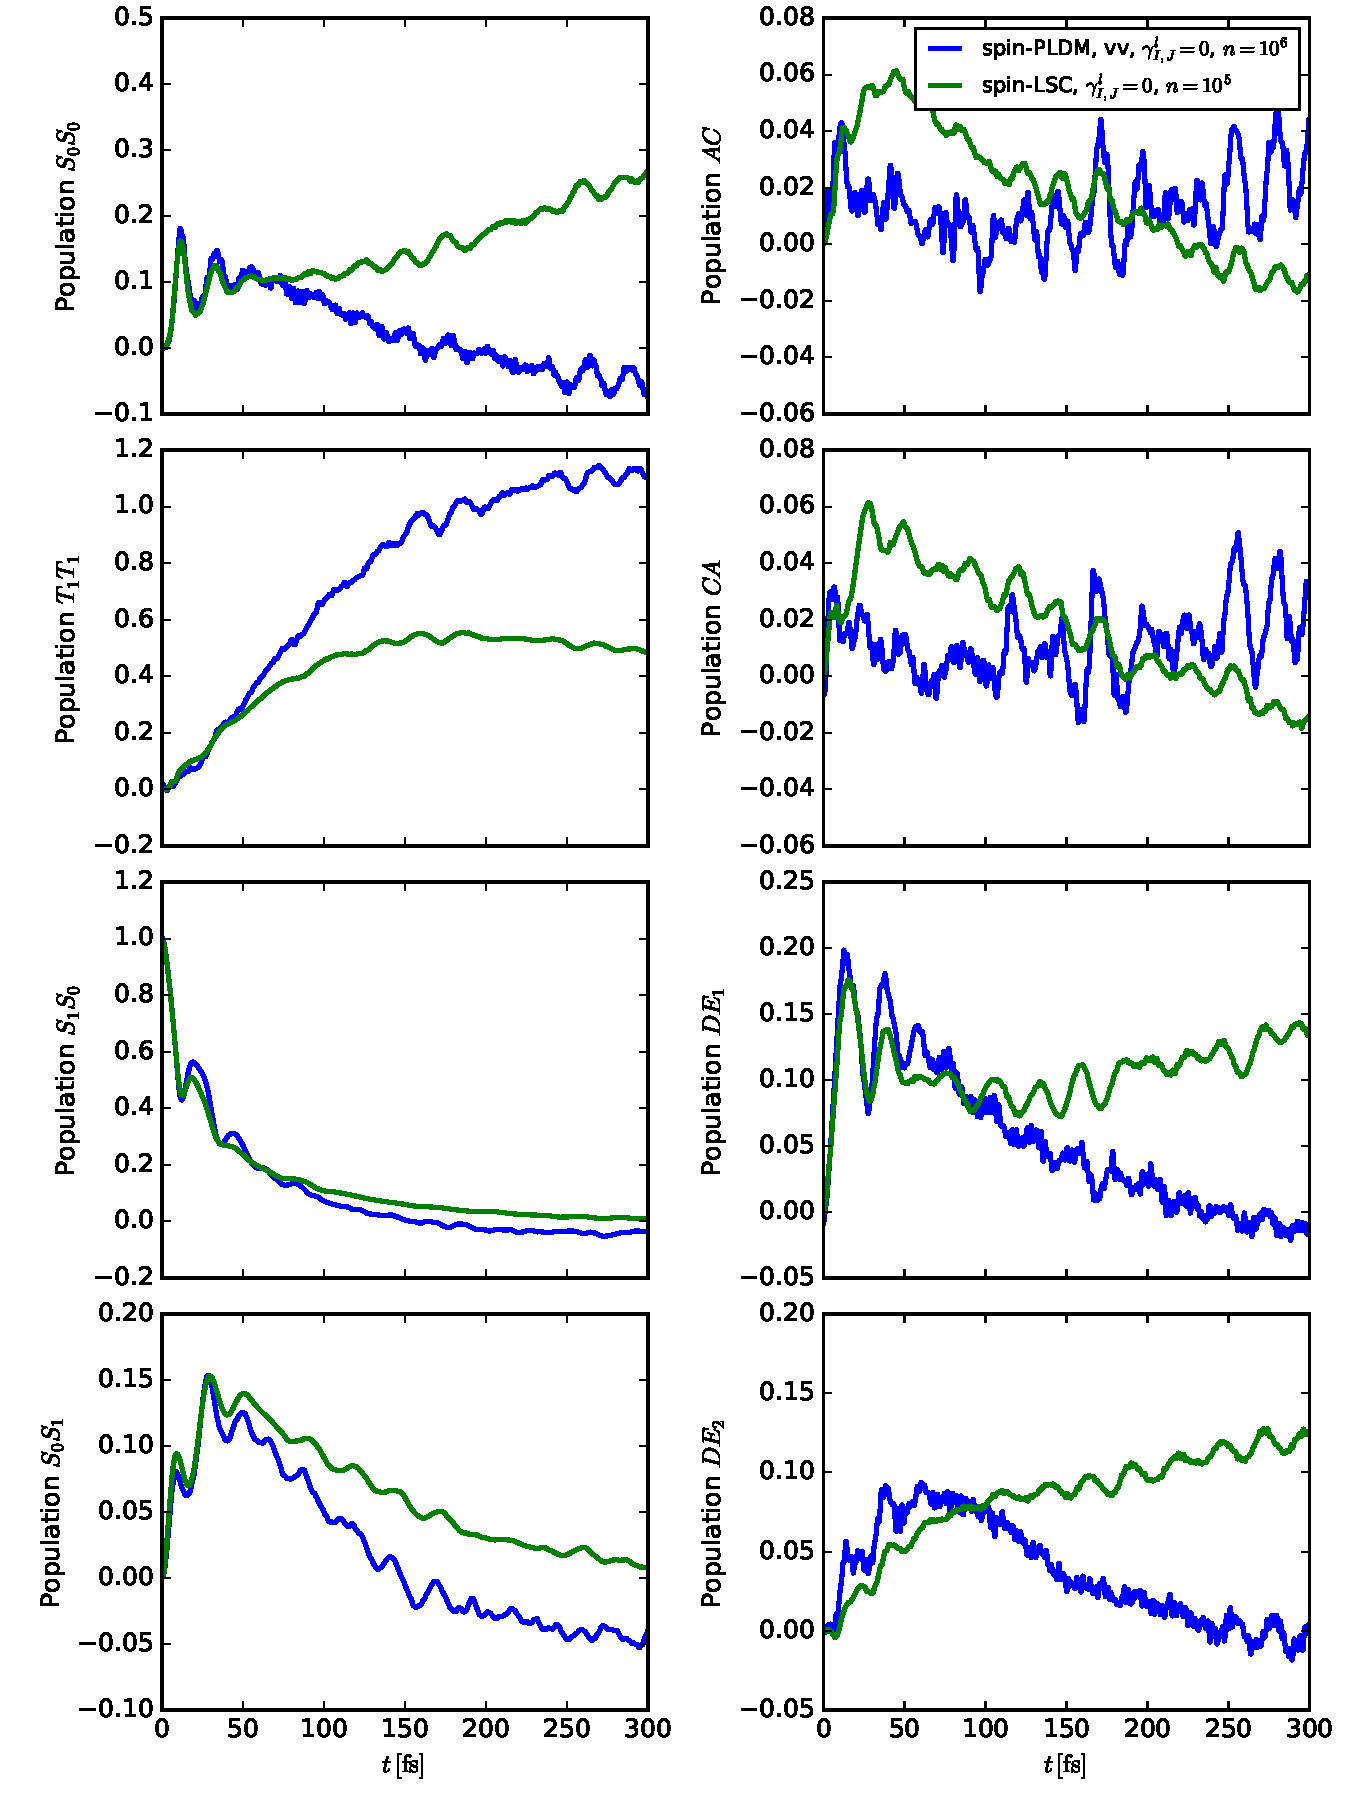
\includegraphics[width=0.8\textwidth]{figs/SF_comparison_multi_allStates_fixed_spinPLDM_spinLSC_noBilinear.pdf}
	\caption{Comparison of population dynamics for the model with bilinear couplings set to zero $\gamma_{I,J}^l = 0$.}\label{fig:SpinPLDM_red_bilinear}
\end{figure}
\clearpage
\begin{figure}[!h]
	\centering
	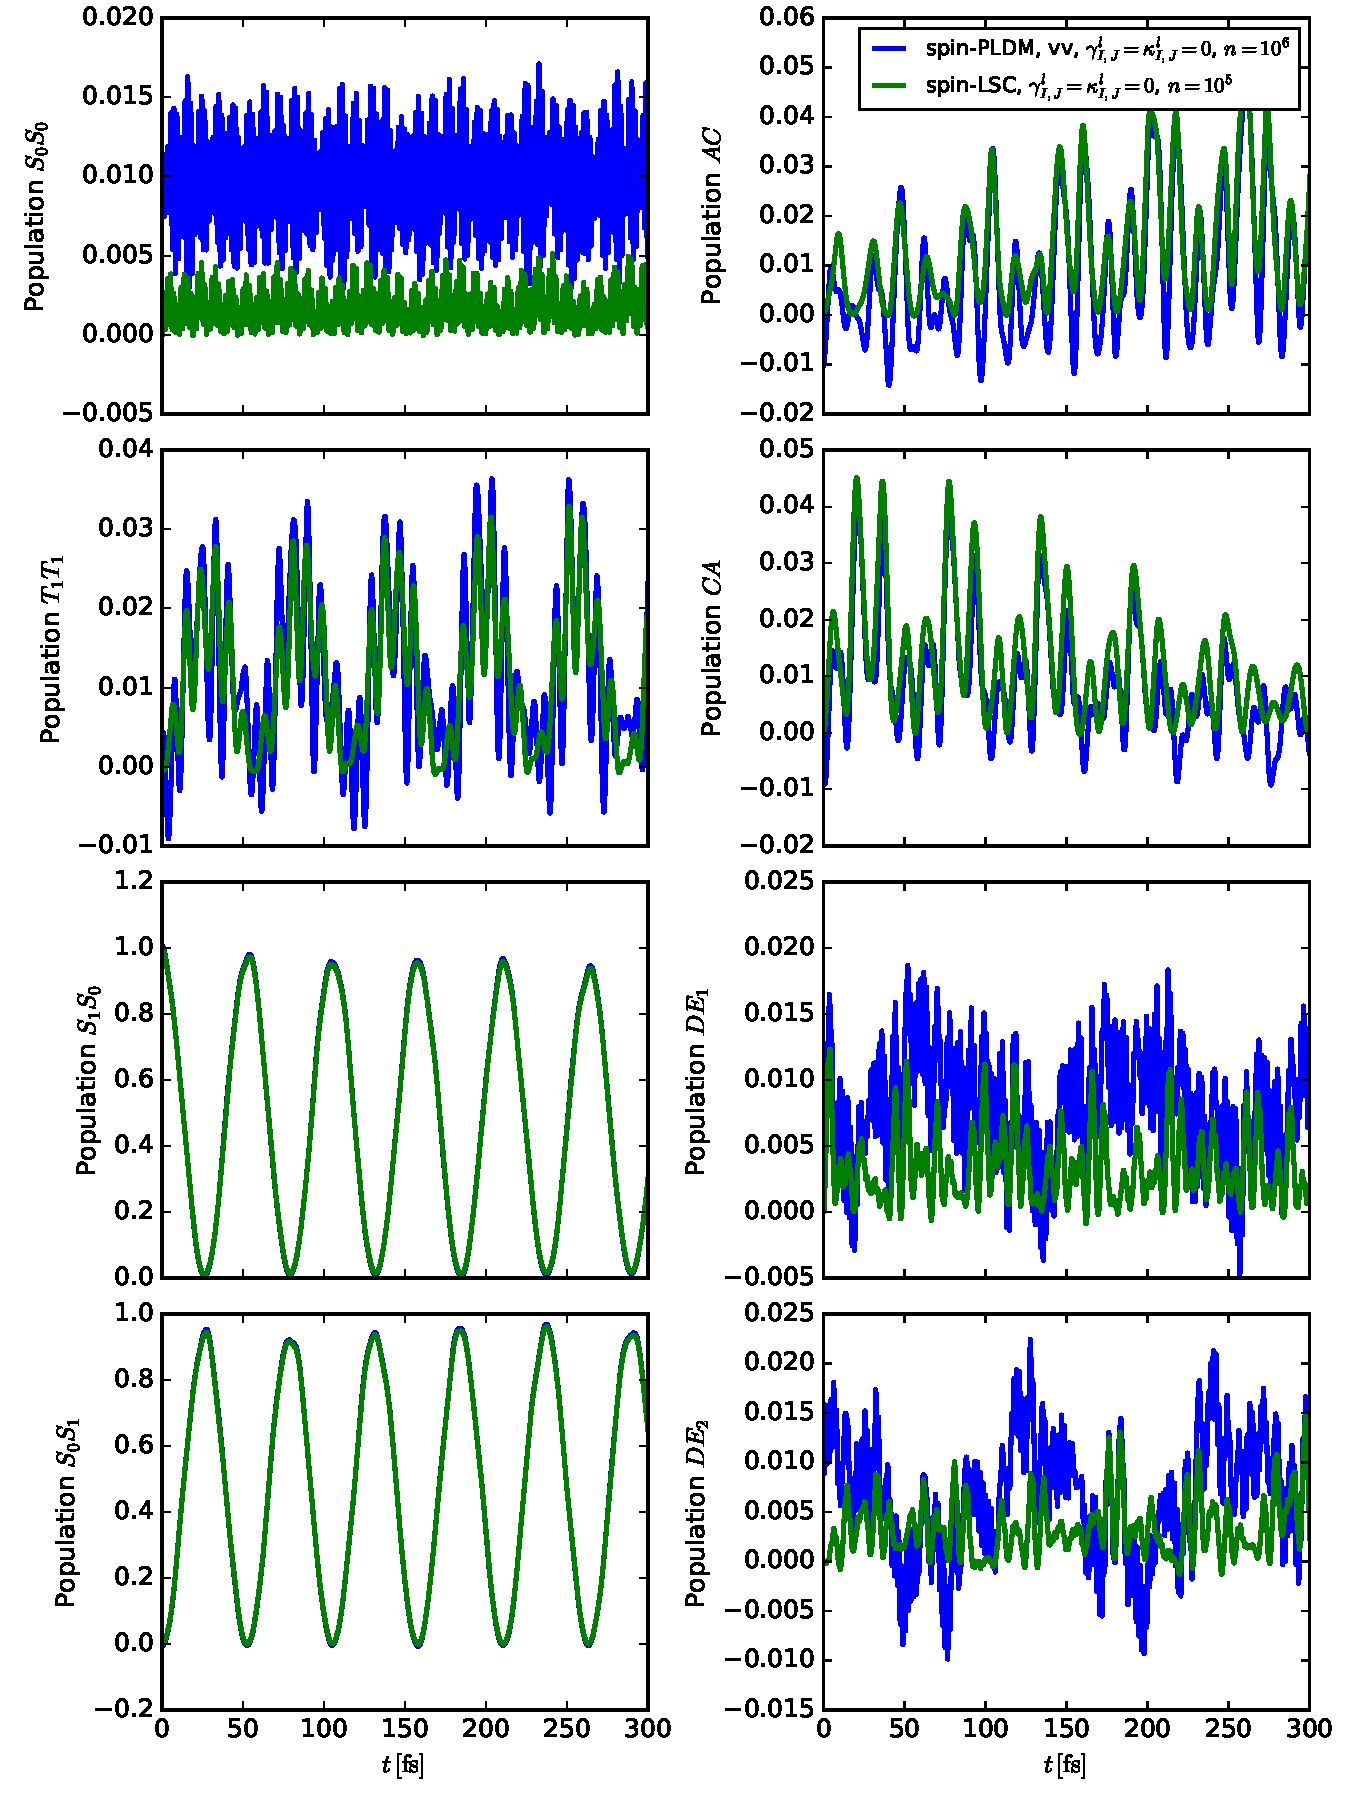
\includegraphics[width=0.8\textwidth]{figs/SF_comparison_multi_allStates_fixed_spinPLDM_spinLSC_noCoupling.pdf}
	\caption{Comparison of population dynamics for the purely electronic model.}\label{fig:SpinPLDM_red_nocoupl}
\end{figure}


\printbibliography
\end{document}


